% https://es.overleaf.com/latex/templates/project-report/jpzczmpsdzwm

%%% Preamble
\documentclass[paper=leter, fontsize=11pt]{scrartcl}
\usepackage[utf8]{inputenc}
\usepackage[spanish,mexico]{babel}
\usepackage[T1]{fontenc}    % use 8-bit T1 fonts
\usepackage{lmodern}
\usepackage{hyperref}       % hyperlinks
\usepackage{lipsum}
\usepackage[square,numbers]{natbib}

\usepackage[protrusion=true,expansion=true]{microtype}	
\usepackage{amsmath,amsfonts,amsthm} % Math packages
\usepackage[pdftex]{graphicx}
\usepackage{url}
 
\usepackage{booktabs}
\usepackage[table,xcdraw]{xcolor}

\usepackage{tikz}
\usetikzlibrary{positioning,matrix, arrows.meta}

\usepackage{caption} 
\usepackage{subcaption}

\usepackage{multirow}

\usepackage{listings}
\lstdefinestyle{mystyle}{ 
    basicstyle=\ttfamily\footnotesize,
    breakatwhitespace=false,         
    breaklines=true,                 
    captionpos=b,                    
    keepspaces=true,                 
    numbers=left,                    
    numbersep=5pt,                  
    showspaces=false,                
    showstringspaces=false,
    showtabs=false,                  
    tabsize=4
}

\lstset{style=mystyle}
\renewcommand{\lstlistingname}{Código}


\selectlanguage{spanish}
\usepackage[spanish,onelanguage,ruled]{algorithm2e}


%%% Custom sectioning
\usepackage{sectsty}
\allsectionsfont{\centering \normalfont\scshape}


%%% Custom headers/footers (fancyhdr package)
\usepackage{fancyhdr}
\pagestyle{fancyplain}
\fancyhead{}											% No page header
\fancyfoot[L]{}											% Empty 
\fancyfoot[C]{}											% Empty
\fancyfoot[R]{\thepage}									% Pagenumbering
\renewcommand{\headrulewidth}{0pt}			% Remove header underlines
\renewcommand{\footrulewidth}{0pt}				% Remove footer underlines
\setlength{\headheight}{13.6pt}


%%% Equation and float numbering
\numberwithin{equation}{section}		% Equationnumbering: section.eq#
\numberwithin{figure}{section}			% Figurenumbering: section.fig#
\numberwithin{table}{section}				% Tablenumbering: section.tab#


%%% Maketitle metadata
\newcommand{\horrule}[1]{\rule{\linewidth}{#1}} 	% Horizontal rule

%%% https://tex.stackexchange.com/a/118217
\usepackage{mathtools}
\DeclarePairedDelimiter\ceil{\lceil}{\rceil}
\DeclarePairedDelimiter\floor{\lfloor}{\rfloor}

\usepackage{amsmath}

\usepackage{tikz}

\title{
		%\vspace{-1in} 	
		\usefont{OT1}{bch}{b}{n}
		\normalfont \normalsize \textsc{Posgrado de Ingeniería de Sistemas} \\ [25pt]
		\horrule{0.5pt} \\[0.4cm]
		\huge Teorema de Bayes para datos de Covid-19 \\
		\horrule{2pt} \\[0.5cm]
}
\author{
		\normalfont 								\normalsize
        Alberto Benavides\\[-3pt]		\normalsize
        \today
}
\date{}


%%% Begin document
\begin{document}
\maketitle

\section{Teorema de Bayes}
Según \citet{grinsteadEA1997}, en problemas en los que hay $m$ hipótesis $H_i, i = [1, m]$ que pueden ser confirmadas por alguna evidencia $E$, se puede utilizar el teorema de Bayes para conocer la probabilidad de una determinada hipótesis dada la evidencia $P(H_i|E)$ según la fórmula
\begin{equation}
    \label{bayes}
    P(H_i|E) = \frac{P(H_i) P(E|H_i)}{\sum_{k = 1}^m P(H_k) P(E|H_k)}.
\end{equation}

\section{Pruebas de detección de Covid--19}

Estos conceptos de la probabilidad se pueden aplicar a ramas de la epidemología donde se usan pruebas para detectar enfermedades. En 2020 se vive una pandemia dada por el contagio del virus SARS--CoV--2, responsable de la enfermedad Covid--19 \citep{stat}. Existen diferentes tipos de pruebas para detectar el contagio presente o pasado de esta enfermedad \citep{fda}, las cuales tienen algunas características \citet{ranjan2020} que ayudan a determinar la posibilidad de que sus resultados sean correctos. En este respecto, existen cuatro posibilidades (véase la tabla \ref{posibilidades} en la p. \pageref{posibilidades}):
\begin{itemize}
    \item Verdadero positivo ($\text{VP}$): El paciente está infectado $p$ y fue diagnosticado positivo $p'$.
    \item Falso positivo ($\text{FP}$): El paciente no está infectado $n$ y fue diagnosticado positivo $p'$.
    \item Falso negativo ($\text{FN}$): El paciente está infectado $p$ y fue diagnosticado negativo $n'$.
    \item Verdadero negativo ($\text{VN}$): El paciente no está infectado $n$ y fue diagnosticado negativo $n'$.
\end{itemize}

% \begin{figure}
%     \centering
%     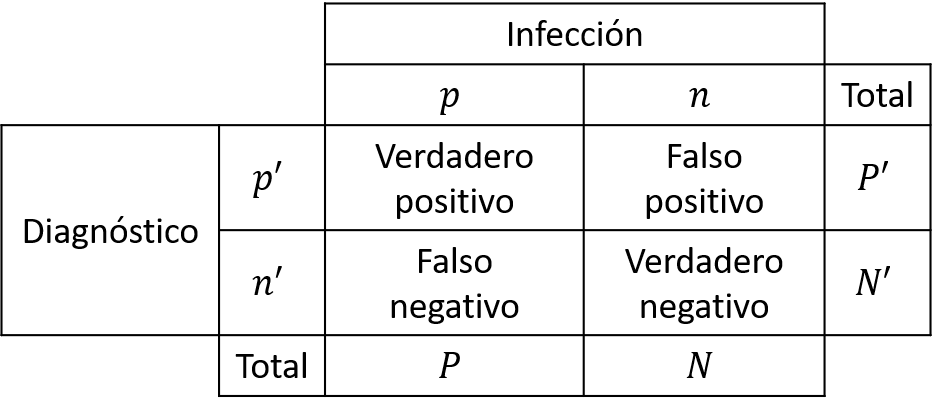
\includegraphics[width=1\textwidth]{img/posibilidades.png}
%     \caption{}
%     \label{posibilidades}
% \end{figure}

\begin{table}[]
    \centering
    \caption{Representación visual de las combinaciones entre diagnóstico e infección de pacientes de Covid--19.}
    \begin{tabular}{cc|c|c|}
    \cline{3-4}
                                                       &      & \multicolumn{2}{c|}{Infección} \\ \cline{3-4} 
                                                       &      & $p$               & $n$        \\ \hline
    \multicolumn{1}{|c|}{\multirow{2}{*}{Diagnóstico}} & $p'$ & Verdadero positivo         & Falso positivo         \\ \cline{2-4} 
    \multicolumn{1}{|c|}{}                             & $n'$ & Falso negativo                & Verdadero negativo         \\ \hline
    \end{tabular}
    \label{posibilidades}
\end{table}

Además, a partir de estas posibilidades se pueden calcular
\begin{itemize}
    \item Exactitud: $\frac{\text{VP} + \text{VN}}{P + N}$,
    \item Precisión: $\frac{\text{VP}}{\text{VP} + \text{FP}}$,
    \item Sensibilidad: $\frac{\text{VP}}{\text{VP} + \text{FN}}$,
    \item Especificidad: $\frac{\text{FN}}{\text{VN} + \text{FP}}$.
\end{itemize}

\section{Datos utilizados}

Con todo esto, se puede aplicar este teorema a valores de contagio obtenidos de datos reales. Se extraen de la Secretaría de Salud de México \citep{gob} datos de contagios de Covid--19 en México. De estos datos se extraen solamente los casos que se consideran positivos y negativos, o sea $p' = 864,696$ positivos y $n' = 1,072,760$ negativos; con un total de $1,937,456$ pruebas.

\section{Exactitud de las pruebas}

Entre las distintas pruebas que existen, el porcentaje de exactitud puede variar desde un $20\%$ a un $80\%$ según las características y tipos de pruebas aplicadas. Los porcentajes más bajos corresponden a pruebas consideradas rápidas que se realizan a partir de muestras de sangre. Los resultados altos para las pruebas se asocian a pruebas virales (de mucosas y tejidos del sistema respiratorio). Para pacientes asintomáticos, las pruebas virales tienen una exactitud de $30\%$ a $50\%$, mientras que en los pacientes con síntomas, están en el rango de $60\%$ a $80\%$ \citep{garcia2020, LisboaEA2516}. Generalmente, el porcentaje de exactitud para pruebas bayesianas que se suele elegir es de $70\%$, por lo que se tomará dicho valor en este análisis también.

\section{Estimaciones a partir de los datos}
De los valores que se tienen a partir de los datos de contagios obtenidos de la Secretaría de Salud de México y del $70\%$ estimado de exactitud de las pruebas, se pueden obtener la cantidad de verdaderos positivos $\text{VP} = 0.7 p'$, falso positivo $\text{FP} = 0.3 n'$, falsos negativos $\text{FN} = 0.3 p'$, y verdaderos negativos $\text{VN} = 0.7 n'$. Esto queda representado en la tabla \ref{carac}. Con estos resultados, se puede estimar el número de contagiados en México es $p = \text{VP} + \text{FN} = 927, 115$, en tanto el número de personas no contagiadas que se hicieron las pruebas sería $n = p = \text{VN} + \text{FP} = 1,010,341$. Estos estimados incrementan un $7.2\%$ los casos positivos y disminuyen un $5.9\%$ los casos negativos, en relación a los reportados.

\begin{table}[]
    \centering
    \caption{Diagnósticos e infecciones a partir de los datos de la Secretaría de Salud de México y el estimado de $70\%$ de exactitud en las pruebas realizadas.}
    \begin{tabular}{c|c|c|}
    \cline{2-3}
                               & $p$       & $n$       \\ \hline
    \multicolumn{1}{|c|}{$p'$} & $605,287$ & $259,409$  \\ \hline
    \multicolumn{1}{|c|}{$n'$} & $321,828$ & $750,932$ \\ \hline
    \end{tabular}
    \label{carac}
\end{table}

\section{Teorema de Bayes aplicado a pruebas de Covid--19}
En el caso de las pruebas de Covid--19, se pueden definir algunas variables. Por ejemplo, $H_1:$ ``estoy contagiado de Covid--19''; $E:$ ``la prueba salió positiva''. De este modo, se podría desear averiguar si un paciente tiene Covid--19 dado que recibió una prueba con resultado positivo, esto es $P(H_1|E)$. Por otro lado, $H_2:$ ``no estoy contagiado de Covid--19''. De aquí, se tiene $P(H_1) = \frac{927,115}{1,937,456} = 0.4785$ como la proporción de pacientes con Covid--19 entre todos los que se hicieron la prueba; y $P(H_2) = 1 - P(H_1) = 0.5215$ en tanto la proporción de pacientes no contagiados de Covid--19 de entre los que se hicieron la prueba.

Así, se pueden obtener algunos otros datos de interés como la proporción de pruebas positivas para los pacientes que sí están infectados $P(E | H_1) = 0.7$ y para los que no lo están $P(E | H_2) = 0.3$.

Con estos valores, se puede calcular $P(H_1 | E)$ a partir de la ecuación \ref{bayes} como sigue:
\begin{equation*}
    P(H_1 | E) = \frac{P(H_1) P(E|H_1)}{P(H_1) P(E|H_1) + P(H_2) P(E|H_2)} = 0.6816,
\end{equation*}
es decir que se tiene una probabilidad de estar contagiado de un $68.16\%$ si es que una prueba sale positiva, a partir de los supuestos aquí descritos.

\section{Notas adicionales}
El teorema de Bayes es una manera de conocer probabilidades de eventos dependientes entre sí que puede aplicarse para dar estimaciones más certeras a partir de resultados observados. En este caso, es posible repetir los cálculos con valores que reflejen la prueba usada para la detección del Covid--19 y sus porcentajes de exactitud asociados, además del número de pruebas realizadas, los casos positivos y negativos, tanto falsos como verdaderos.

\bibliographystyle{espnat}
\bibliography{Biblio}

\end{document}